\documentclass[french]{rapport}
\usepackage{josty}

\usepackage{amsmath,amsthm}
\usepackage[ruled]{algorithm2e}

\usepackage{tikz}
\usetikzlibrary{positioning}
\usetikzlibrary{arrows}


\newcommand{\fun}[1]{\texttt{#1}}

\begin{document}

\title{Jobshop : Méthodes approchées}
\subtitle{Compte-rendu du projet de TP «~Optimisation Combinatoire~»}
\author{Joseph Boudou}
\date{14 janvier 2013}
\maketitle

\section{Présentation}

Dans le cadre du projet de travaux pratiques du cours d'optimisation combinatoire, nous avons
développé un programme de résolution du problème de jobshop par des méthodes approchées. Différentes
heuristiques ont été implémentées, notamment un algorithme génétique. Cette métaheuristique a été
préférée à la recherche tabou qui était aussi proposée. En effet, les algorithmes génétiques nous
intriguaient, en particulier leur aptitude à diversifier les solutions pour sortir des mimima locaux
ainsi que les caractérisques nécessaire à l'opération de mutation afin que l'algorithme soit
efficace.

Le programme a été développé en langage \texttt{C}. Ce langage nous à paru approprié dans la mesure
où il produit des exécutables rapides. D'autre part, les structures de données nécessaires à
l'implémentation nous semblaient assez simples pour être implémentées dans ce langage qui ne possède
pas de biblothèque standart proposant des structures génériques. Pour l'utilisation du logiciel
produit, nous renvoyons le lecteur à la page de manuel l'accompagnant.

L'intérêt de ce travail étant pédagogique, certaines solutions implémentées mais n'ayant finalement
pas été retenues sont tout de même présentées. Ainsi, nos choix et leur motivations sont présentés
et nous pouvons rendre compte des recherches que nous avons menées.

La section suivante présente la méthodologie utilisée pour évaluer les algorithmes implémentés,
cette problématique étant essentielle pour la mise au point d'un algorithme génétique. La section
\ref{sec:codage} expose la représentation des solutions qui a été utilisée. Les sections
\ref{sec:greedy}, \ref{sec:vois} et \ref{sec:gen} présentent ensuites les différents algorithmes
implémentés, respectivement l'heuristique gloutonne, la descente locale et l'algorithme génétique.
Enfin, une conclusion est donnée à la section \ref{sec:conc}. Les résultats expérimentaux des
différents algorithmes sont donnés tout au long de ce rapport.

\section{Évaluation des algorithmes}

L'évaluation des algorithmes produits a été nécessaire tout au long du projet. Elle nous a permis de
faire les choix parmis les nombreuses alternatives possibles. Cependant cette évaluation est assez
difficile puisque les résultats dépendent fortement de l'instance traitée d'une part et du hasard
d'autre part puisque la majorité des algorithmes sont stochastiques.

Les deux paramètres principaux pris en compte sont le makespan et la durée du calcul. Le nombre
d'itération nous est rapidement apparus comme une donnée arbitraire dont la signification varie trop
fortement suivant les paramètres des algorithmes. L'occupation de l'espace mémoire est difficile à
mesurer par l'application elle-même. Nous avons parfois utiliser des outils externes pour en avoir
une approximation mais il n'a pas été possible d'automatiser cette mesure. Le nombre de voisins
générés et le nombre de croisements effectués nous a beaucoup servis pour fixer de nombreux paramètres de
l'algorithme génétique. Il n'ont cependant pas beaucoup de sens pour la comparaison des algorithmes
entre eux, le temps de traitement étant une valeur plus objective.

Afin de comparer les algorithmes entre eux, notamment dans ce rapport, nous avons donc calculé, pour
chaque instance traitée, l'efficacité de l'algorithme par rapport aux meilleurs resultats connus
$$
 \mathit{Eff} = \frac{F(\hat{x})}{\mathit{best\_known\_result}}
$$
La moyenne de cette efficacité ainsi que l'écart type, le minimum et le maximum sont donnés. D'autre
part, le même genre de calcul a été effectué avec le resultat d'autres algorithmes. Nous appelons
cette mesure l'\emph{efficacité relative}
$$
  \mathit{Eff_{relative}} = \frac{F(\hat{x})}{F(\hat{y})}
$$
où $\hat{y}$ est la meilleure solution de l'algorithme par rapport auquel la comparaison est faite.
Comme précédemment, la moyenne, l'écart type, le minimum et le maximum de ces valeurs est donné. Il
est à noter cependant que ces valeurs ne sont pas toutes l'inverse de l'efficacité relative où le
rôle des algorithmes est échangé. Il nous est donc paru utile de donner les deux valeurs. Enfin, le
même genre de calcul est effectué pour le temps de traitement.

En ce qui concerne la variabilité aléatoire des algorithmes stochastiques, le programme réalisé
permet de répéter le calcul plusieurs fois. Les valeurs affichées sont alors des
moyennes. Cependant, certains algorithmes sont particulièrement lents et le calcul du jeu complet
d'instance prend un temps important. Pour les résultats présentés dans ce rapport, les algorithmes
stochastiques n'ont donc été répétés que deux fois.


\section{Codages}

Les solutions sont représentées par les permutations des jobs pour chaque ressource. Cette
représentation a l'avantage d'être simple et intuitive. Elle permet de s'assurer que toutes les
solutions représentent des solutions actives. À chaque solution active correspond une seule
représentation. Cependant toutes les représentations ne correspondent pas à une solution admissible.
Il est possible qu'il y ait interbloquage.

D'autre part cette représentation ne permet pas de calculer facilement le makespan. Lors de la
construction d'une solution à partir de l'instance du problème il est toujours possible de calculer
le makespan. Mais si la solution est modifiée (par exemple en permutant deux tâches) l'incidence sur
le makespan ne peut être calculée directement et la solution doit être \emph{rejouée}
(\fun{plan\_replay}).

\newcommand{\st}{\mathit{st}}

Afin d'accélérer certaines opérations (en particulier le calcul des voisinages) un certain nombre
d'informations sont conservées pour chaque tâche, en plus de l'identifiant du job. Ces informations
précisent la date de début de la tâche ($\st_{(i,j)}$), sa durée ($p_{(i,j)}$) et la date de fin de
l'opération précédente ($\st_{(i-1,j)} + p_{(i-1,j)}$).
Ces informations ne sont bien
entendue pas affichée dans la solution fournie à l'utilisateur.

Dans la suite de ce document $r_{kt}$ représente l'indice $j$ de la $t$\textsuperscript{ième} tâche de la ressource
$k$ pour la solution considérée et $R = \cup{\left\{r_{kt}\right\}}$.


\section{Heuristique gloutonne}

L'heuristique implémentée est de type «~Earliest Due Date~» (EDD).

\newcommand{\sr}{\mathit{sr}}
\newcommand{\so}{\mathit{so}}

On note $\sr_k$ la date de fin de la dernière tâche programmée pour la ressource $k$. On sélectionne
pour chaque job la prochaine opération disponible :
$$ \forall j,~d_j = \min_{(i,j) \notin R} i $$
Pour chacune de ces opérations on détermine la date possible de lancement
$$ \forall j,~\so_j = \max (\st_{(d_j-1,j)} + p_{(d_j-1,j)}, \sr_{k_{(d_j,j)}}) $$
Ensuite on ne garde que les opérations dont la date $\so_j$ est minimale
$$ S_1 = \left\{ j ~|~ \so_j = \min_{j'} {\so_{j'}} \right\} $$
On calcule la durée restante de travail pour chaque job de $S_1$
$$ \forall j \in S_1,~ W_j = \sum_{i \geq d_j}{p_{(i,j)}} $$
Et on ne garde que les jobs dont la durée restante est maximale
$$ S_2 = \left\{ j \in S_1 ~|~ W_j = \max_{j' \in S_1}{W_{j'}} \right\} $$
Enfin, au cas où $S_2$ ne serait pas un singleton, on sélectione le job d'indice maximum
$$ j^* = \max S_2 $$
On affecte alors $(d_{j^*}, j^*)$ à sa ressource et on recommence la procédure tant que toutes les
opérations n'appartiennent pas à $R$



\section{Voisinages et recherches locales}

\subsection{Voisinage par transposition adjacente admissible}

Le mouvement dans l'espace des solutions envisagé pour construire le voisinage d'une solution est la
transposition de deux tâches adjacentes dans une des permutations correspondant à une ressource. Un
tel voisinage aurait $m (n - 1)$ éléments, dont certains ne correspondraient pas à une solution
admissible. Afin d'éliminer ces inconvénients une transposition $((i,j),(i',j'))$ n'est acceptée que
si $i' = 0$ ou si la fin de l'opération $(i',j')$ précéde la fin de l'opération $(i,j)$ :
\begin{equation} \label{eq:admis_transp}
  \st_{(i'-1,j')} + p_{(i'-1,j')} < \st_{(i,j)} + p_{(i,j)}
\end{equation}

Nous allons montrez que l'inéquation (\ref{eq:admis_transp}) interdit d'obtenir une solution non
admissible à partir d'une solution admissible. Dans la représentation d'un problème de jobshop par
un graphe orienté, la transposition de deux tâches adjacentes correspond au changement de sens d'un
seul arc disjonctif. De même, l'interblocage est caractérisé par un cycle dans le graphe. Si le
graphe d'origine $G$ ne possède pas de cycle mais que le changement de sens d'un arc $\alpha = (i,j)
\rightarrow (i',j')$ introduit un cycle, alors il existe un chemin $C$ de $(i,j)$ à $(i',j')$ ne
passant pas par $\alpha$. Soit $G_k$ le sous-graphe de $G$ ne contenant que les nœuds utilisant la
ressource $k$ et tel que $\alpha$ soit un arc de $G_k$. $G_k$ est la représentation d'un ordre
total. En raison de la transitivité et comme $G$ n'est pas cyclique, $C$ ne contient aucun arc de
$G_k$. On en déduit que l'arc $(i'-1,j) \rightarrow (i',j')$ appartient à $C$ et donc 
$$ \st_{(i'-1,j')} \geq \st_{(i,j)} + p_{(i,j)} $$
Ce qui contredit l'inéquation (\ref{eq:admis_transp}) puisque $p_{(i'-1,j)} > 0$.

D'autre part, les transpositions ne verifiant pas (\ref{eq:admis_transp}) ne peuvent pas produire
une solution dont le makespan est inférieur à celui de l'original. En effet, l'arc $\alpha$ ne peut
pas appartenir au chemin de poid maximum. Si c'était le cas, le chemin entre la
source et le nœud $(i',j')$ passant par $(i,j)$ devrait avoir au moins le même poid que le chemin
entre la source et $(i',j')$ passant par $(i'-1,j')$.

Le voisinage obtenu contient encore beaucoup de voisins. Il a été constaté expériementalement que le
filtre proposé n'élimine qu'environs $\frac{1}{5}$ des transpositions possibles. Et inversement, la
distance entre les voisins est relativement petite, puisqu'ils ne diffèrent que par deux gènes. Ce
voisinage permet donc une exploration assez exhaustive, mais risque d'être facilement bloqué par le
moindre minimum local.


\subsection{Algorithme de descente locale}

L'algorithme de descente locale implémenté utilise le voisinage par transposition adjacente
admissible présenté précédemment. Bien que ce voisinage possède de nombreux voisins, le mouvement
correspondant est relativement élémentaire et il le moindre col stoppe la descente. Nous avons donc
choisi d'utiliser la solution fournie par l'algorithme glouton pour initialiser la recherche.


\subsection{Voisinage par réduction du chemin critique}

Le voisinage utilisé jusqu'ici est de type \emph{meilleur d'abord}. Tous les voisins sont générés et
le meilleur de ces voisins est gardé. Nous avons aussi réalisé un voisinage de type
\emph{premier d'abord} pour lequel un seul voisin est généré. Le mouvement élémentaire reste le
même, une transposition adjacente admissible, mais une heuristique est utilisée afin de sélectionner
un mouvement prometteur. En l'occurence, l'heuristique implémentée tente de choisir un arc sur le chemin
de poid maximum dont le changement de sens permettrait une réduction du makespan.

Pour cela, on recherche la dernière periode d'inactivité de la première ressource $k$ dont le
makespan est maximum. La tâche succédant cette période d'inactivité pour la ressource $k$ est une
opération $(i,j)$. On parcours alors toutes les opérations $(i',j)$ en commençant par $i' = i$
jusqu'à $i' = 0$. La première transposition admissible d'une opération $(i',j)$ avec une opération
la précédant sur sa ressource est sélectionnée.

Le calcul de ce voisinage est bien entendu beaucoup plus rapide que le voisinage \emph{meilleur
d'abord}. Cependant, les objectifs ne sont pas atteints. Premièrement, la méthode utilisée ne garanti
pas que l'arc sélectionné soit bien sur un chemin critique. Deuxièmement, même si l'arc sélectionné
est sur un chemin critique, son changement de sens peut amener le makespan à augmenter. Enfin,
l'analyse du comportement de ce voisinage sur les instances à traiter montre qu'il boucle très
rapidement sur un petit ensemble de solutions.

L'algorithme de descente locale implémenté avec ce voisinage prend en compte ces limitations. La
meilleure solution trouvée $\hat{x}$ est stockée séparément de la solution courante $x$ et des
solutions moins satisfaisante que $\hat{x}$ sont acceptée. L'algorithme s'arrête lorsque $m + n$
itérations succéssives n'ont pas permis d'améliorer $\hat{x}$.

Les résultats obtenus par rapport à l'algorithme de descente locale précédent (voir tableau
\ref{tab:local2}) sont légèrement moin bon en ce qui concerne le makespan et bien meilleur en ce qui
concerne le temps de calcul. Cependant, les temps de calcul de l'algorithme précédent étaient
déjà suffisament courts. 

\subsection{Algorithme VNS}

Bien que non-demandée dans le projet de TP, l'implémentation d'une heuristique de recherche locale
de la famille des \emph{Variable Neighbourhood Search} (VNS) nous a semblé à la fois évidente et
facile compte tenu du voisinage choisi. Le principe de cette métaheuristique est d'effectuer une
descente locale en alternant différents voisinages.

Le voisinage par transposition adjacente admissible peut être limité aux transpositions des tâches
d'une seule ressource. On obtient alors un ensemble de voisinages $V_k$ pour $0 \leq k < m$. Le
principe de l'algorithme implémenté est présenté par l'Algo. \ref{algo:VNS}. La valeur initiale de
la solution $\hat{x}$ est fournie par l'heuristique gloutonne.

\begin{algorithm}[bt]
  \SetKwFunction{MS}{makespan}
  \SetKw{modulo}{modulo}

  \KwIn{une solution admissible $\hat{x}$}

  $x \leftarrow \hat{x}$ \;
  $k \leftarrow 0$ \;
  $c \leftarrow 0$ \;
  \While{$c < m$}{
    $x \leftarrow \arg \min_{y \in V_k(x)}{\MS{y}} $ \;
    \uIf{$\MS{x} < \MS{\ensuremath{\hat{x}}}$}{
      $\hat{x} \leftarrow x$ \;
      $c \leftarrow 0$ \;
    }
    \lElse{
      $c \leftarrow c + 1$ \;
    }
    $k \leftarrow (k + 1) \mod m$ \;
  }
  \caption{VNS}
  \label{algo:VNS}
\end{algorithm}

Cette heuristique est particulièrement efficace, comme le montre la Tableau \ref{tab:VNC}. Elle est
en mesure de rivaliser avec l'algorithm génétique tout en étant bien plus rapide (jusqu'à plus de
1\,000 fois).



\section{Algorithme génétique}

\subsection{Opérateur de mutation}

Nous avons réutilisé les voisinages par transposition adjacente admissible limités à une ressource
$V_k$ définis précédemment. L'operateur de mutation choisi consiste à prendre toutes les solutions
dans un voisinage $V_k$, $k$ étant choisi au hasard. Cet opérateur est assez différent des
opérateurs habituels de mutation dans la mesure où il fourni une importante quantité de solutions
pour un seul individu (autours de $\frac{4(n-1)}{5}$). Pour revenir dans un schéma plus classique
nous aurions pu appliquer une recherche locale qui nous aurait fourni une solution unique. Cependant
nos résultats expérimentaux nous ont montré que l'opérateur de mutation choisi ne permettait très
souvent de s'éloigner de minimum locaux qu'en passant par des voisins aillant un makespan important.

Nos expérimentations nous ont aussi amenés à privilégier les cas où le voisinage $V_k$ choisi
correspond à une ressource dont le makespan est maximum. Nous avons ainsi contraint la probabilité
qu'un tel $k$ soit choisi afin qu'elle soit toujours supérieure ou égale à $\frac{1}{8}$.

Afin d'évaluer cet opérateur, nous avons implémenté une variante de notre algorithme génétique qui
ne réalise que des mutations (aucun croisement). Les résultats, présentés dans le Tableau
\ref{tab:mutations}, montrent clairement qu'un tel algorithme converge vers une bonne solution.
D'autre part, l'opération de mutation est plus rapide que l'opérateur de croisement.



\subsection{Opérateur de croisement par ordre partiel}

Le premier opérateur de croisement implémenté consiste à construire des enfants pour lesquels
l'ordre des tâches pour chaque ressource respecte l'ordre partiel commun aux deux parents. Pour cela
on construit pour chaque parent et chaque ressource $k$ un graphe orienté dont les nœuds sont les jobs
ayant une opération sur la ressource et dont les arcs $j \rightarrow j'$ sont étiquetés par $-1$ si le
job $j$ précède le job $j'$ et par $1$ s'il le succède. La matrice d'incidence est calculée pour
chaque graphe ainsi construit.
Par exemple, aux permutation des jobs $R_0 = (0,3,1,2)$ et $R_1 = (3,2,0,1)$ correspondent les
matrices :
\begin{align*} 
  M_0 &= \begin{pmatrix}
   0 &  1 &  1 &  1 \\
  -1 &  0 &  1 & -1 \\
  -1 & -1 &  0 & -1 \\
  -1 &  1 &  1 &  0
  \end{pmatrix} &
  M_1 &= \begin{pmatrix}
   0 &  1 & -1 & -1 \\
  -1 &  0 & -1 & -1 \\
   1 &  1 &  0 & -1 \\
   1 &  1 &  1 &  0
  \end{pmatrix}
\end{align*}

On calcule alors l'ordre partiel en faisant la moyenne des deux matrices obtenues.
Par exemple :
$$ M = \frac{M_0 + M_1}{2} = \begin{pmatrix}
   0 &  1 &  0 &  0 \\
  -1 &  0 &  0 & -1 \\
   0 &  0 &  0 & -1 \\
   0 &  1 &  1 &  0
\end{pmatrix} $$
Cette matrice correspond à l'ordre partiel suivant :
\begin{center}
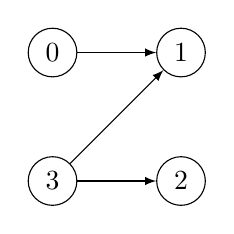
\begin{tikzpicture}[>=latex,every node/.style={draw,circle}]
  \node (n0)               {0} ;
  \node (n1) [right=of n0] {1} ;
  \node (n2) [below=of n1] {2} ;
  \node (n3) [below=of n0] {3} ;
  \draw [->] (n0) -- (n1) ;
  \draw [->] (n3) -- (n1) ;
  \draw [->] (n3) -- (n2) ;
\end{tikzpicture}
\end{center}

On construit alors aléatoirement des descendants qui respectent cet ordre partiel. Par exemple, à
partir de l'ordre précédent on peut construire les descendants $R'_0 = (3,0,1,2)$ et $R'_1 =
(0,3,2,1)$.

Cet opérateur de croisement permet une bonne intensification puisqu'il conserve le maximum de ce qui
est commun aux parents. D'autre part, puisqu'il est stochastique, il devrait permettre une certaine
diversification. Cependant, en pratique, cet opérateur s'est montré peu efficace. D'une part il est
relativement lent. D'autre part, ses actions d'intensification et de diversification ne s'appliquent
pas dans les bonnes situations. Lorsque la population est très diverse et qu'il y a donc besoin
d'intensification, l'ordre partiel est très mince (voire vide) et l'opérateur s'apparente à une
génération aléatoire. Inversement, lorsque la population est très homogène et qu'il y a donc besoin
de diversification, l'ordre partiel est presque total et les solutions générées sont très semblables
à leurs parents.

Nous avons donc cherché un autre opérateur de croisement. Cependant, afin de pouvoir évaluer ce
nouvel opérateur, il est toujours possible d'expérimenter cet opérateur de croisement. Une variante
de l'algorithme génétique ne différent que par l'opérateur de croisement est disponible et donne les
résultats lisibles dans le Tableau \ref{tab:order}.


\subsection{Opérateur de croisement à un point}

Nous avons donc implémenté l'opérateur classique de croisement à un point adapté aux permutations.
Cet opérateur consiste à déterminer aléatoirement un pivot compris entre 0 et la taille $n$ de la
permutation. Pour des raisons d'efficacité, nous avons choisi de limiter l'intervale de choix du
pivot à $\left[ \lfloor \frac{n}{4} \rfloor, n - \lfloor \frac{n}{4} \rfloor \right]$. Ensuite
toutes les valeurs à gauche du pivot dans le second parent sont supprimées du premier parent. De même
les valeurs à droite du pivot dans le premier parent sont supprimées du second parent. Les valeurs
restantes sont décalées à droite pour le premier parent et à gauche pour le second. Enfin la partie
à gauche du pivot dans le second parent est collée dans le premier et la partie droite du premier
parent est copiée dans le second. La figure \ref{fig:onepoint} résume ces différentes étapes.

\begin{figure}[htb]
  \centering
  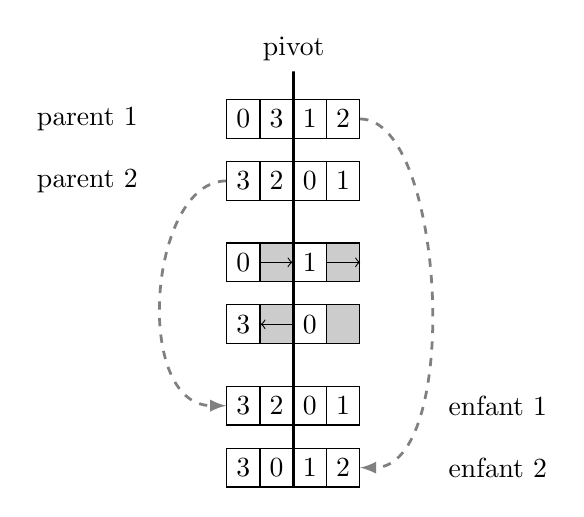
\begin{tikzpicture}
    [every node/.style={draw,minimum width=1.2em,minimum height=1.4em,node distance=1.2em}]

    \tikzstyle{grey}  = [fill=black!20]
    \tikzstyle{label} = [draw=none]

    \node (a0) {0} ;
    \node [right of=a0] (a1) {3} ;
    \node [right of=a1] (a2) {1} ;
    \node [right of=a2] (a3) {2} ;

    \node [below=0.8em of a0] (b0) {3} ;
    \node [right of=b0] (b1) {2} ;
    \node [right of=b1] (b2) {0} ;
    \node [right of=b2] (b3) {1} ;

    \node [below=1.5em of b0] (c0) {0} ;
    \node [right of=c0,grey]  (c1) {} ;
    \node [right of=c1] (c2) {1} ;
    \node [right of=c2,grey] (c3) {} ;

    \node [below=0.8em of c0] (d0) {3} ;
    \node [right of=d0,grey] (d1) {} ;
    \node [right of=d1] (d2) {0} ;
    \node [right of=d2,grey] (d3) {} ;

    \node [below=1.5em of d0] (e0) {3} ;
    \node [right of=e0] (e1) {2} ;
    \node [right of=e1] (e2) {0} ;
    \node [right of=e2] (e3) {1} ;

    \node [below=0.8em of e0] (f0) {3} ;
    \node [right of=f0] (f1) {0} ;
    \node [right of=f1] (f2) {1} ;
    \node [right of=f2] (f3) {2} ;
    
    \draw [line width=1pt] (a1.north east)
                        -- +(0,1em) node [label,anchor=south] {pivot}
                        -- (f1.south east);

    \draw [->] (c0) -- (c2) ;
    \draw [->] (c2) -- (c3.east) ;
    \draw [->] (d2) -- (d0) ;

    \draw [-latex,dashed,line width=1pt,color=black!50]
          (a3) .. controls +( 1.3,0) and +( 1.3,0) .. (f3.east) ;
    \draw [-latex,dashed,line width=1pt,color=black!50]
          (b0) .. controls +(-1.2,0) and +(-1.2,0) .. (e0.west) ;

    \node [label,left=1 of a0] {parent 1} ;
    \node [label,left=1 of b0] {parent 2} ;
    \node [label,right=1 of e3] {enfant 1} ;
    \node [label,right=1 of f3] {enfant 2} ;
  \end{tikzpicture}
  \caption{Opérateur de croisement à un point}
  \label{fig:onepoint}
\end{figure}
 
Contrairement à l'opérateur précédent, l'opérateur de croisement à un point conserve un grand nombre
d'informations même lorsque les chromosomes sont très différents. En effet, dans tous les cas, si
une tâche en précéde une autre dans un enfant, elle la précédait forcement dans au moins un des
parents. En pratique, les résultats du tableau \ref{tab:genetic} montrent que cet opérateur de
croisement est d'une part plus rapide, d'autre part plus efficace que l'opérateur précédent. Nous
avons essayé d'utiliser les deux opérateurs de croisement conjointement mais, quelle que soit la
proportion de chaque opérateur que nous avons essayée, nous n'avons jamais obtenu de résultats
meilleurs que lorsque l'opérateur de croisement à un point est utilisé seul.


\subsection{Opérateur de sélection}

\newcommand{\op}{\mathit{op}}
\newcommand{\mut}{\mathit{mutation}}
\newcommand{\co}{\mathit{crossover}}

Les individus d'une populations sont classés selon la valeur du makespan. Afin de sélectionner les
individus devant être mutés ou croisés, la population est traversée du meilleur makespan au plus
long. La probabilité d'une opération (mutation ou croisement) est calculée selon la formule
\begin{equation} \label{eq:proba}
 P_r = \frac{c_\op}{(h-r)q_\op} \times \frac{F\left( \frac{h}{2} \right)}{F(r)}
\end{equation}
où $r$ est le rang de l'individu dans la population, $c_\op$ le nombre d'enfants qu'on souhaite
encore obtenir par l'opération $\op$, $h$ la taille de la population, $q$ le nombre d'enfants que
l'opération $\op$ crée et $F$ la function qui associe au rang d'un individu son makespan. La valeur
$c_\op$ est actualisée après que chaque individu de la population parent a été considéré.

Nos diverses tentatives nous ont incités à favoriser les mutations, en particulier lorsque
l'algorithme se trouve piégé dans un minimum local. La valeur initiale de $c_\mut$ (avant de
considerer le meilleur individu d'une nouvelle population) dépend donc du nombre $\mathit{im}$ de générations
n'ayant pas amélioré la meilleure valeur du makespan connue. Les valeurs pour (\ref{eq:proba}) sont
\begin{align*}
  c_\mut &= \min \left(h \left( \frac{1}{4} + \frac{\mathit{im}}{g} \right) , h \right) \\
  q_\mut &= \frac{4}{5} (n-1)
\end{align*}
$g$ étant le nombre maximum autorisé de générations successives n'améliorant pas le makespan
(condition d'arrêt). Ainsi la probabilité d'une mutation est faible lorsqu'une nouvelle meilleure
solution est trouvée et elle augmente progressivement tant que cette solution n'est pas remplacée.

Afin d'obtenir à chaque itération le même nombre $h$ d'enfants, la probabilité de réaliser un
croisement dépend de la probabilité de réaliser une mutation. D'autre part, afin de ne pas croiser
plusieur fois le même couple de solutions pour la même génération, les croisements d'un individu de
rang $r$ ne sont envisagés qu'avec des individus de rang inférieur. Les valeurs pour
(\ref{eq:proba}) sont
\begin{align*}
  c_\co &= h - c_\mut \\
  q_\co &= 2 \left( h - (r + 1) \right)
\end{align*}


\subsection{Opérateur de construction}

Nous utilisons un opérateur élitiste considérant les parents et les enfants.  Afin de générer une
nouvelle génération $G_{u+1}$ à partir de la génération précédente $G_u$ et des enfants $E_u$, les
$h$ meilleurs individus sont sélectionnés parmis les individus de $E_u$ et les $\frac{h}{4}$
meilleurs de $G_u$. En cas d'égalité, les enfants sont privilégiés. Les doublons sont éliminer ce
qui peut amener à ajouter des individus supplémentaires de $G_u$ afin que $G_{u+1}$ comporte bien
$h$ solutions. Cet opérateur a l'avantage de toujours conserver la meilleure solution trouvée.

\subsection{Autres paramètres}

La première génération $G_0$ est peuplée par la solution de l'heuristique gloutonne et par des
solutions admissible aléatoires.

La taille $h$ de la population est fixée à 1\,024. Comme l'opérateur de construction est élitiste,
le nombre d'individus doit être suffisant pour conserver les mauvaises solutions permettant de
franchir les cols. Cependant une taille plus importante ralentit l'algorithme.

L'algorithm s'arrête lorsque la limite $g$ du nombre d'itérations successives sans amélioration de la
meilleure solution est atteint. Ce nombre est fixé à 512.


\subsection{Améliorations}

Les deux opérateurs de croisement proposés peuvent produire des solutions qui ne sont pas
admissibles. Une fonction de réparation des solutions non-admissibles a donc été implémentée. La
solution est rejouée et lorsqu'un interblocage est détecté, une permutation permettant de briser le
cycle dans le graphe est réalisée. Ainsi toutes les solutions générées par chacun des opérateurs
conduisent à une solution admissible. Cette amélioration a permis d'accélérer notablement
l'algorithme en réduisant le nombre d'exécution des opérateurs de croisement. D'autre part,
les permutations effectuées renforcent la diversification.

\section{Conclusion}

Les résultats obtenus par les différents algorithmes restent bien sûr bien loin des meilleurs
résultats connus pour une importante partie des instances proposés. Cependant, sur certaines
instances de difficulté moyenne (par exemple la31), nous avons pu constaté une amélioration
consistante du makespan et du temps de calcul tout au long du projet.

En ce qui concerne l'algorithme génétique, nous avons pu comparer deux opérateurs de mutations et
mieux comprendre les qualités que l'on peut attendre d'un tel opérateur. Mais surtout nous avons pu
constater l'importance primordiale du codage des solutions qui conditionne les opérateurs possibles.
Le changement de codage demande malheureusement beaucoup de travail

\end{document}

% vim: tw=100
